\subsection{Ca sử dụng xem danh sách địa điểm được gợi ý}
\vspace{0.5cm}


\noindent 
\begin{tabularx}{\linewidth}{| l | X |} 
\hline 
\textbf{Mô tả} & Người dùng xem danh sách địa điểm du lịch gợi ý cho bản thân và tùy chỉnh sở thích về loại hình du lịch để lấy gợi ý khác.  \\ 
\hline 
\textbf{Luồng cơ bản} & 1. Người dùng truy cập tab khám phá  \newline
                        2. Người dùng bấm vào trang đề xuất địa điểm du lịch. \newline
                        3. Hệ thống điều hướng đến trang hiển thị danh sách địa điểm du lịch gợi ý cho người dùng và bộ lọc tùy chỉnh. \\
                     
\hline 
\textbf{Luồng thay thế} & Người dùng tùy chỉnh bộ lọc sở thích loại hình du lịch để nhận gợi ý khác.\\           
\hline 
\textbf{Tiền điều kiện} & - Người dùng đang đăng nhập và phiên đăng nhập chưa kết thúc. \newline
                          - Người dùng có thông tin về sở thích. \\
\hline 
\textbf{Hậu điều kiện} & - Người dùng có thể chọn địa điểm trong danh sách để xem chi tiết. \\

\hline 
\textbf{Yêu cầu phi chức năng} & Hệ thống xử lý lấy danh sách không quá 2s  \\ 
\hline 
\end{tabularx}

\vspace{0.8cm}

\noindent 
\begin{tabular}{| c | c |}
    \hline
    \textbf{Biểu đồ hoạt động} & \textbf{Quan hệ} \\ 
    \hline
    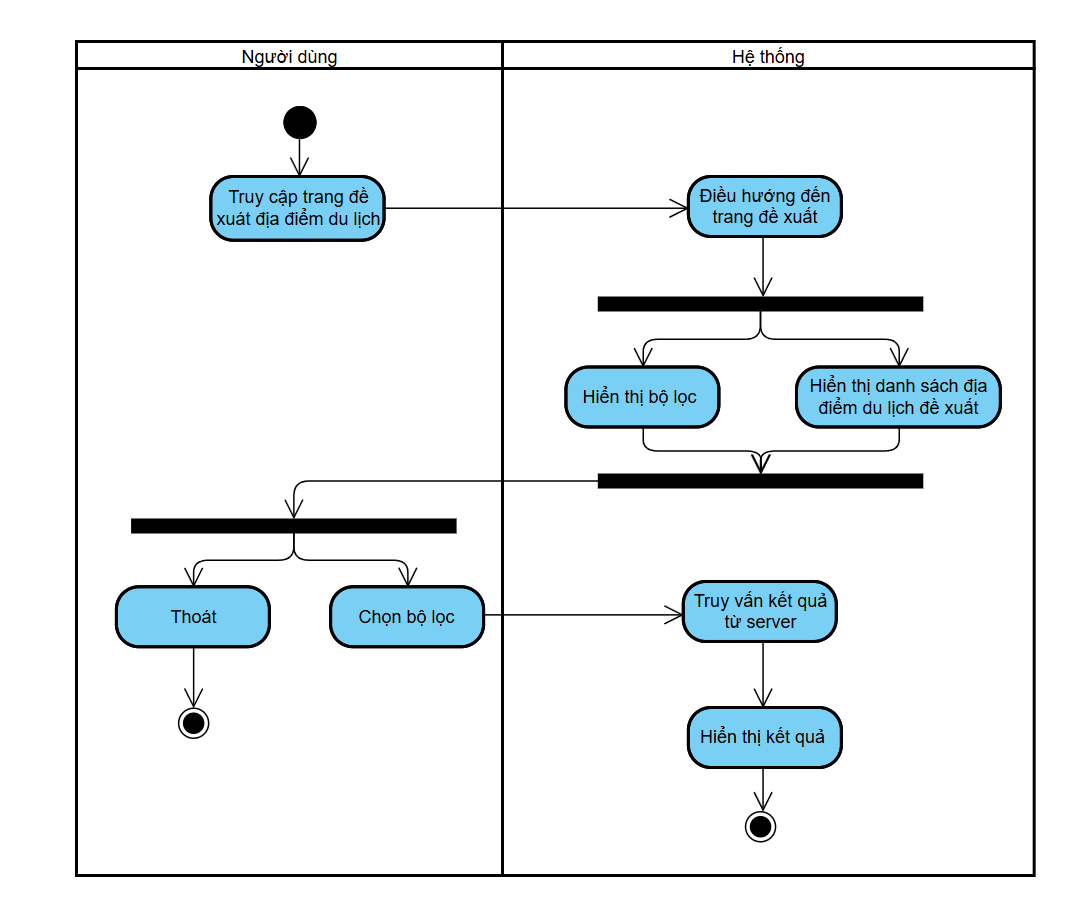
\includegraphics[width=0.5\linewidth]{figures/c3/3-3-6-ad.png} 
    & 
    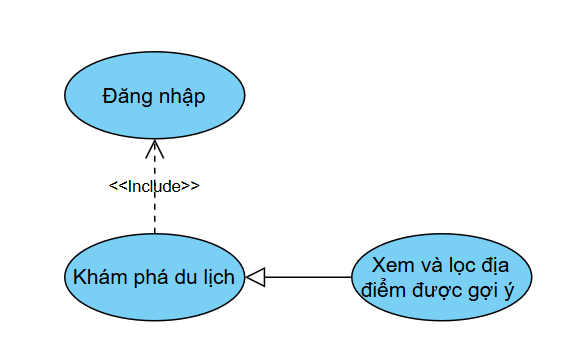
\includegraphics[width=0.45\linewidth]{figures/c3/3-3-6-rd.png} \\ 
    \hline
\end{tabular}



\begin{figure}[H]
    \centering  
    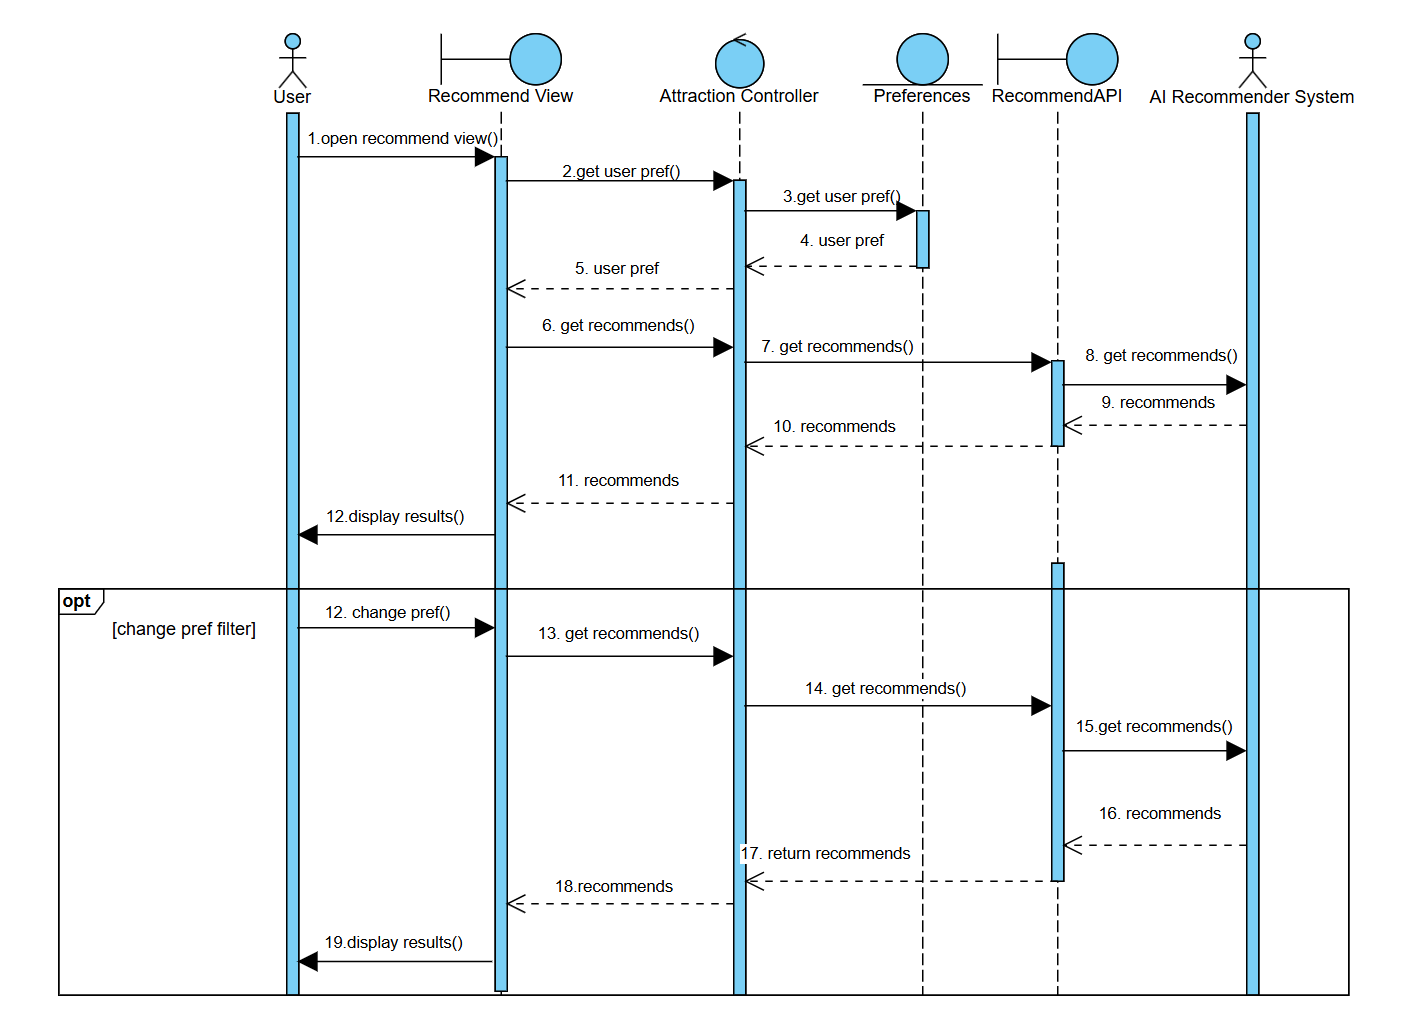
\includegraphics[width=1\textwidth]{figures/c3/3-3-6-sd.png}
    \caption{Biểu đồ tuần tự ca sử dụng xem danh sách địa điểm được gợi ý.}
    \label{fig:3-3-6-sequence-diagram}
\end{figure}